\section{Nominal algorithm}
\label{sec:nominal}
\begin{figure}[!htpb]
  \begin{center}
    \includegraphics[width=0.48\textwidth]{figures/cartoon_roads_small_nominal.pdf}
    \includegraphics[width=0.48\textwidth]{figures/cartoon_roads_large_nominal.pdf}
  \end{center}
  \vspace{-10pt}
  \caption{Sketch of the road coverage of the nominal MMTP algorithm, for a small chamber closest to the beamline (left) and large chamber farthest from the beamline (right). The $X$ road is horizontal, the $U$ road is pink and slanted, and the $V$ road is blue and slanted. The x-axis and y-axis are in units of strip pitches, which are set to be 0.4 mm.}
  \label{fig:cartoon_nominal}
\end{figure}
The MMTP algorithm in its current form is described in \cite{mmtp}. We encourage the reader to begin there. In addition, there are a few details which we will elaborate on in this section.
\par As a reminder, the MMTP relies on the concept of roads to form coincidences for a trigger. The wedge is divided into roads which define a set of strips on each plane. The MMTP receives ART hits and places them in the corresponding road. The MMTP looks for a coincidence of a fixed number of planes with hits in a road, within the ART time collection window.
\par Each implementation of the MMTP algorithm covers  a fixed but to-be-determined number of roads. For this study, we will use region sizes of 136 roads and 96 roads for the 2.2 m long strips and 0.5 m long strips, respectively. The motivation for these region sizes is further discussed in Section \ref{sec:stereoroads}. 
\begin{figure}[!htpb]
  \begin{center}
    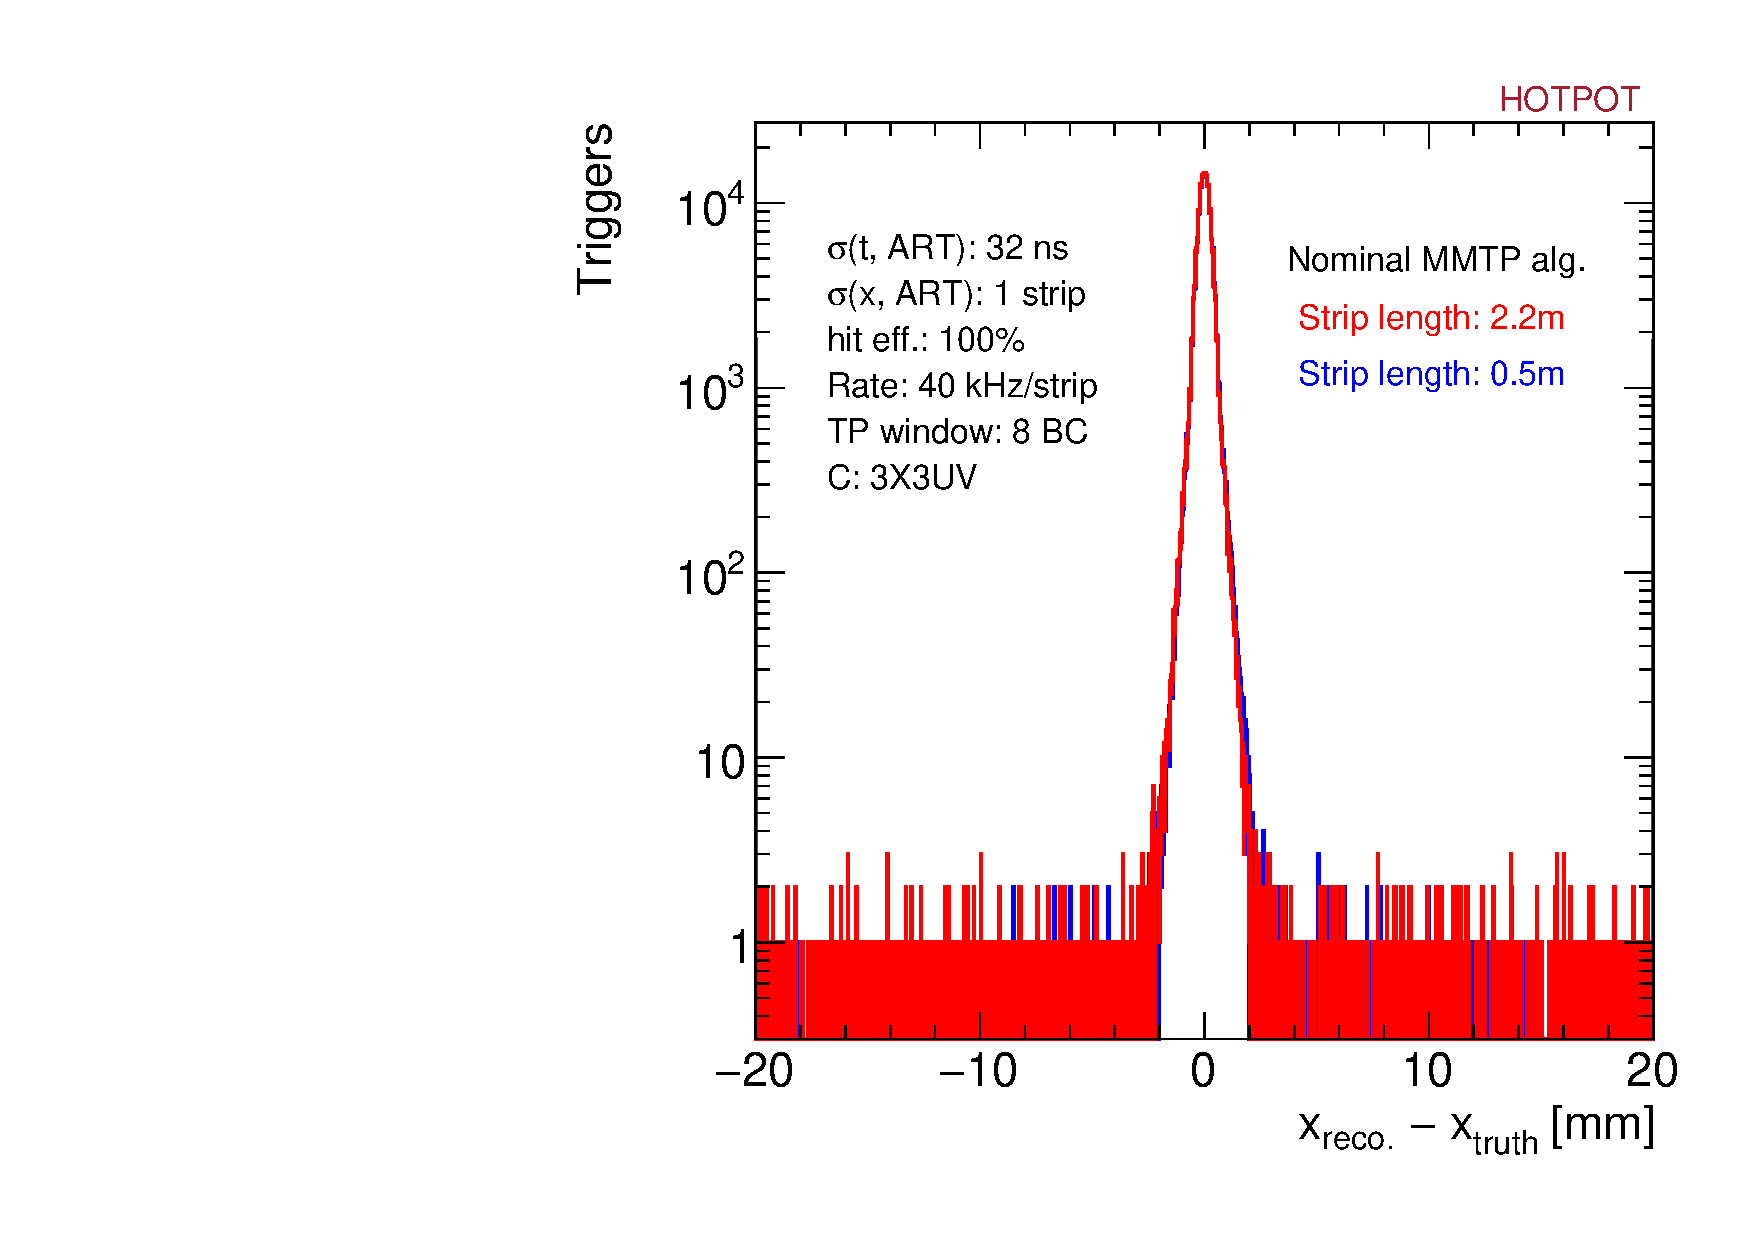
\includegraphics[width=0.48\textwidth]{figures/xres_old.pdf}
    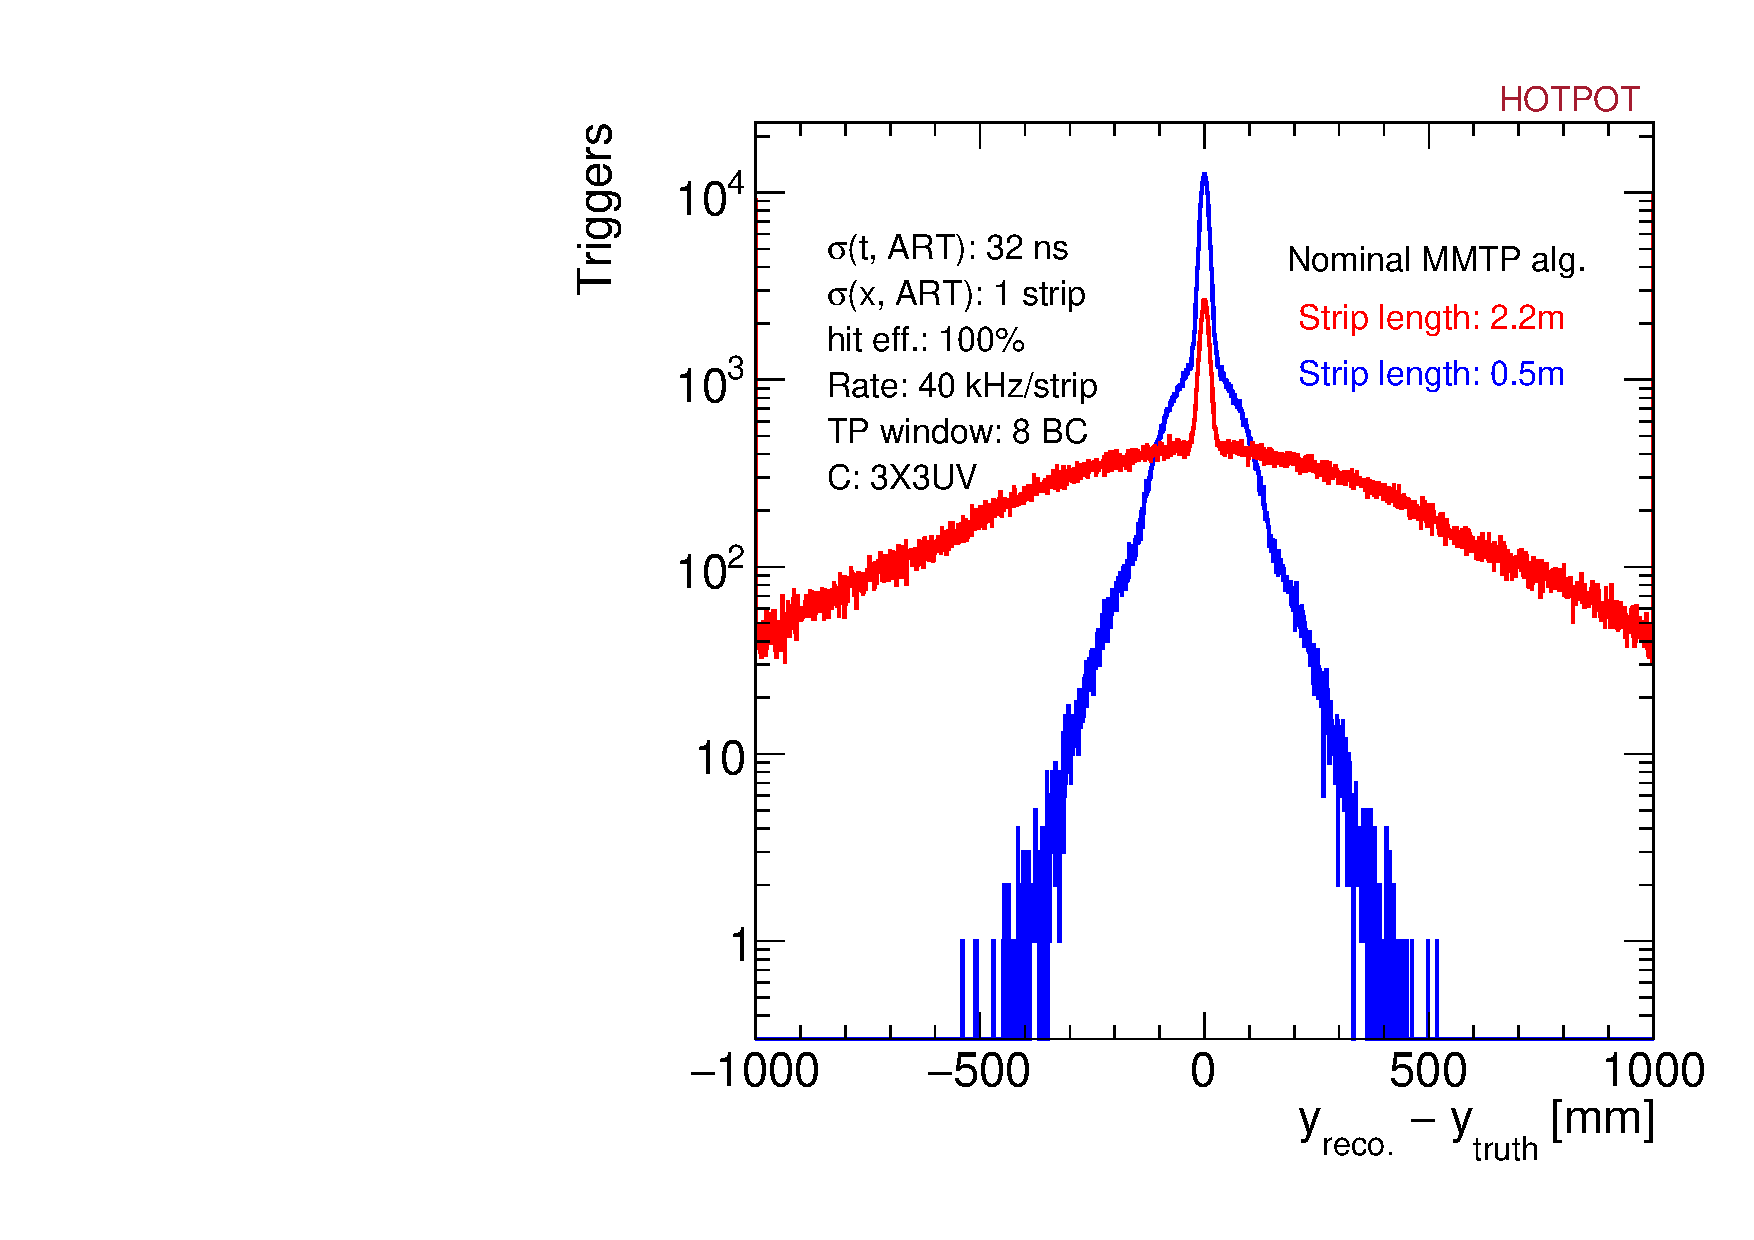
\includegraphics[width=0.48\textwidth]{figures/yres_old.pdf}
    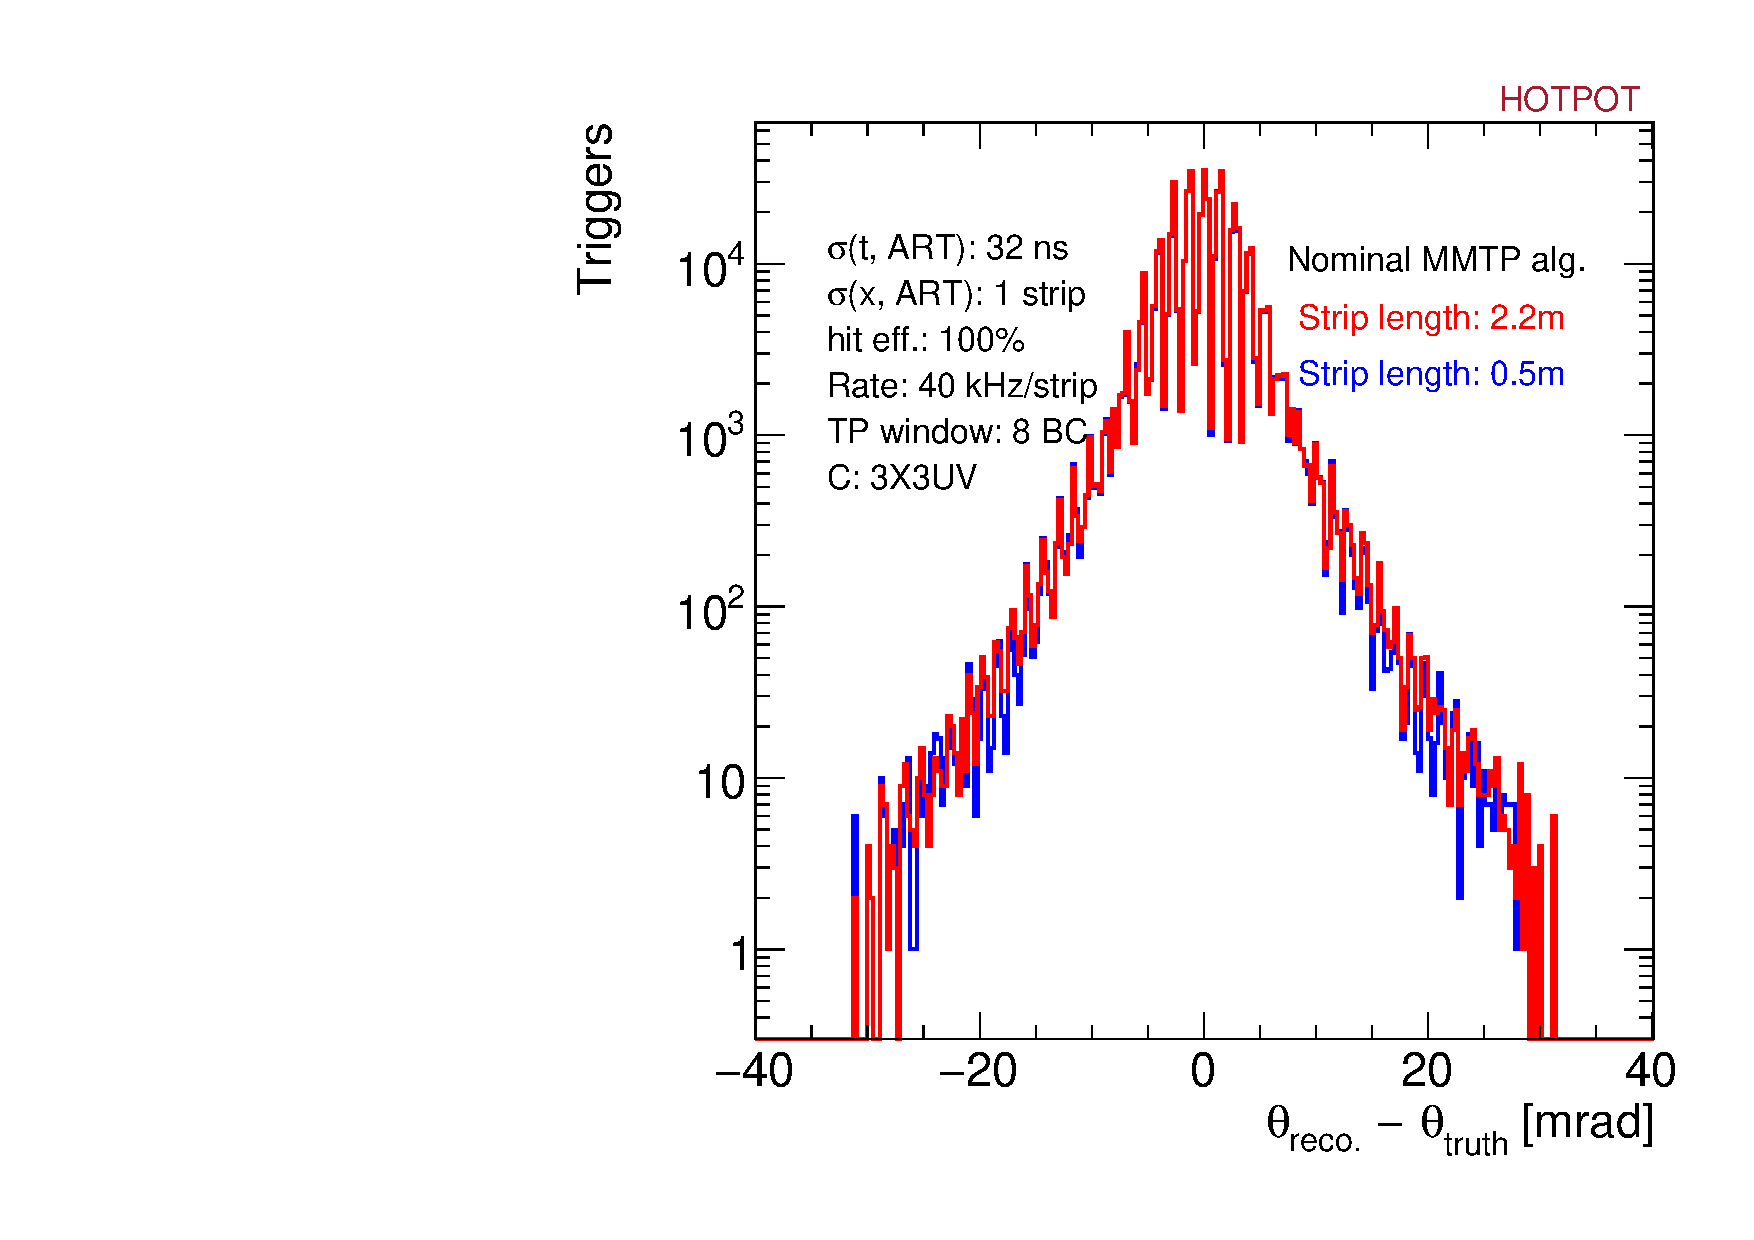
\includegraphics[width=0.48\textwidth]{figures/mres_old.pdf}
  \end{center}
  \vspace{-10pt}
  \caption{Distribution of $x_\text{reco.} - x_\text{truth}$ (top, left), $y_\text{reco.} - y_\text{truth}$ (top, right) and $\theta_\text{reco.} - \theta_\text{truth}$ (bottom) for the nominal MMTP algorithm with uncorrelated background at a rate of 40 kHz per strip.}
  \label{fig:resolutions_old}
\end{figure}
\par Each road spans a certain number of strips on the eight planes in a wedge. The $X$ road size is the number of strips each road spans on on an x plane, and similar definitions apply to the $U$ road size and the $V$ road size. \par To mitigate edge effects when a track spans two roads, each road also sees any hits on ``neighboring" roads (described in more detail in \cite{mmtp}). We note here that we only need to look for hits on one neighboring road to fix these cases, as opposed to both neighboring roads. Furthermore, we modify the scheme so that each road can only see hits on half of the neighboring road. For example, an $X$ road of 8 strips also sees any hits on the adjacent 4 strips. 
\par The $U$,$V$ road size is determined by the $X$ road size. In order for a $U$ or $V$ road to overlap spatially with the entire $X$ road, the $U$,$V$ road size must be larger or equal to the number of strips in an $X$ road plus the number of strips in a neighbor, plus $\tan 1.5^\circ \times \frac{ \text{strip length} }{ \text{strip pitch} }$. Figure \ref{fig:cartoon_nominal} illustrates the effect of the stereo angle on the $U$,$V$ road size.


Figure \ref{fig:resolutions_old} shows the resolution of the MMTP triggers using the nominal algorithm. The reconstructed x position residuals, where x is the precision coordinate, is a narrow distribution bounded by the small $X$ road size, but the reconstructed y resolution is very poor. The RMS calculated in the 3$\sigma$ range of the distribution is 433.4 $\pm$ 0.4 mm for 2.2m long strips. For 0.5m long strips, the 3$\sigma$ RMS is 55.59 $\pm$ 0.05 mm. With a high rate of background, the size of the $U$, $V$ roads makes the trigger extremely vulnerable to background hits. On average, 1.7 stereo plane hits in the track are from background events. In addition, an important consequence of the use of roads in the MMTP algorithm is that each road can only record one ART hit per plane per BC collection window. With large $U$,$V$ roads, a background hit can easily cause the loss of a real muon hit. 
